
In this section, the application of the system for implementation, integration and test is described in detail.
The goal of this plan is to eliminate integration risks and to have the final system do what it is supposed to after one has put together all subsystems.
The activities reported in this category are planned activities and shall be performed in the development and validation process. 

\subsection{Implementation Strategy}

The system will be constructed as an ensemble of loosely coupled components. Each module will represent a certain role in the architecture.
Components will communicate through well-defined interfaces. This modular approach will support parallel development and simplify testing. External services, like routing or weather providers will be accessed through
specialized interfaces, which will reduce coupling and serve to improve testability.

\subsection{Feature Identification}

This section lists the key features of the system which will drive integration and testing work. When the complete behavior is correct, a feature will be marked as done
and then back through the backend to user interface.

The identified features will include:
\begin{itemize}
    \item user management, including registration and authentication;
    \item trip recording and review;
    \item manual contribution of path information;
    \item issue detection and validation;
    \item path search and visualization;
    \item aggregation and moderation of community data.
\end{itemize}

These will be used to characterize the representative integration threads and system-level test scenarios.


\subsection{Component Testing}

Component testing will verify the behavior of individual components in isolation,
before any form of system-level integration is performed.

\paragraph{Visual Conventions.}
The following visual conventions are used in this section. Software components or subsytems are shown as rectangular boxes.
Solid-line boxes represent components which are actually implemented and running.
Dashed-line boxes illustrate stubs (simulated components are employed during testing to
replace external dependencies.
Control or Data flow are represented with arrows between components and indicate the direction of invocation.

Colors are only used to make the text more readable and do not carry any further semantics or architectural constraints.

During component testing, all external dependencies of the component under test will be replaced by stubs.
The number of stubs is not fixed and depends on the number of external dependencies:
one stub will be introduced for each external system that is not part of the
component under test.

Figure~\ref{fig:component_testing} illustrates the planned component testing setup.
The figure shows a test driver invoking the component under test, while all external
dependencies are simulated using stubs.
This setup will be used in testing the internal logic of the component without depending on outside systems like databases or third-party services.

\begin{figure}[H]
    \centering
    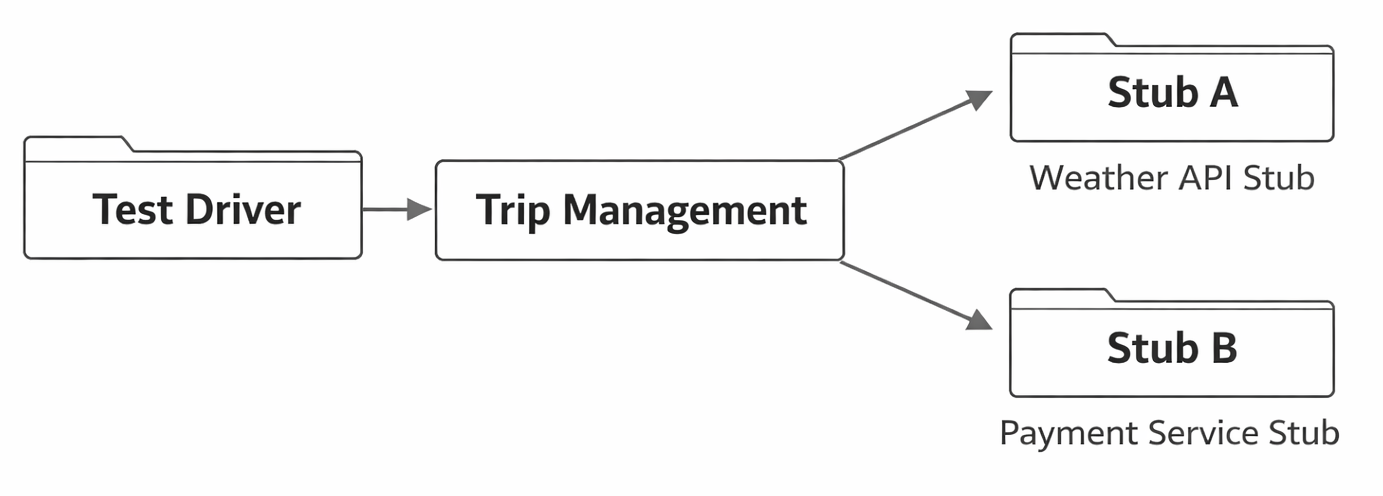
\includegraphics[width=0.85\textwidth]{Figures/component_testing}
    \caption{Component testing using a test driver and stubs.}
    \label{fig:component_testing}
\end{figure}

The caller of the component under test will be simulated by a test driver and will trigger its operations. Stubs will return predefined responses and will make tests deterministic and
repeatable.

%---------------------------------------------------------

\subsection{Incremental Integration Strategy}

After component testing, system integration will be performed incrementally.
Subsystems will not be integrated all at once.

Figure~\ref{fig:incremental_integration} shows the planned incremental integration strategy.
Integration will proceed through successive steps, where the number of real subsystems
will gradually increase.
In early steps, only core infrastructure will be real, while other subsystems and
external services will be replaced by stubs.
As integration progresses, stubs will be progressively replaced by real components.

This approach will make it possible to identify integration problems early and
to limit the impact of faults during later development stages.

\begin{figure}[H]
    \centering
    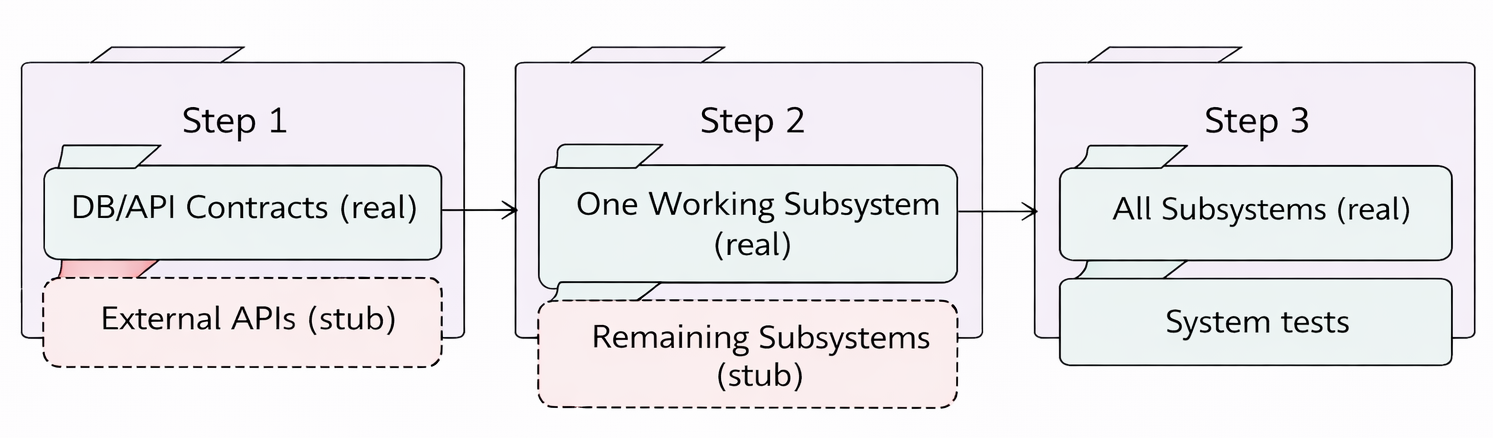
\includegraphics[width=0.9\textwidth]{Figures/incremental_integration}
    \caption{Incremental integration strategy with progressive replacement of stubs.}
    \label{fig:incremental_integration}
\end{figure}

%---------------------------------------------------------

\subsection{Thread-Based Integration}

Apart from this incremental integration, a thread-based integrated approach will be adopted.

A thread is a coherent visible to the user operation that ranges many
components.
Thread-based integration will focus on validating full execution paths rather
than individual subsystems.

Figure~\ref{fig:thread_integration} illustrates the integration of a representative
thread, namely the Path Search and Visualization feature.
The diagram illustrates how the client interface, backend services, stateful storage and any external services collaborate to deliver a single functionality.

This thread will be tested to allow verification of interactions across all involved components and should identify the issues which cannot be detected via
component testing alone.

\begin{figure}[H]
    \centering
    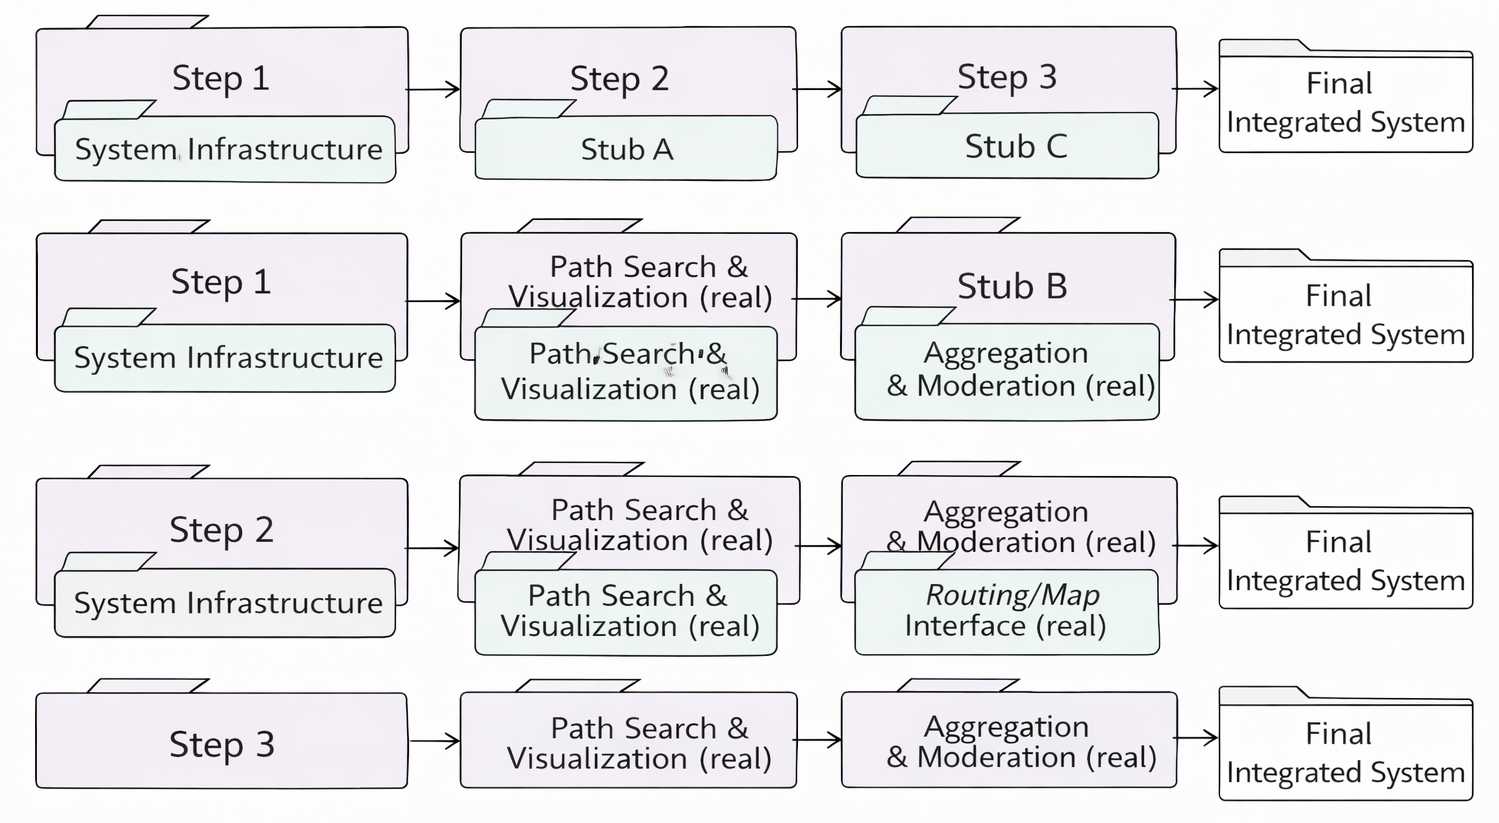
\includegraphics[width=0.9\textwidth]{Figures/thread_integration}
    \caption{Thread-based integration of the Path Search and Visualization feature.}
    \label{fig:thread_integration}
\end{figure}

%---------------------------------------------------------

\subsection{Final System Integration}

Once all subsystems and representative threads are integrated, the system will
reach its final configuration.

Figure~\ref{fig:final_integration} presents the fully integrated system.
At this stage, all components will be real and no drivers or stubs will be used.
The figure represents the system as it will be executed in production.

System testing will be performed on this configuration in order to validate
overall system behavior and interactions from the user's perspective.

\begin{figure}[H]
    \centering
    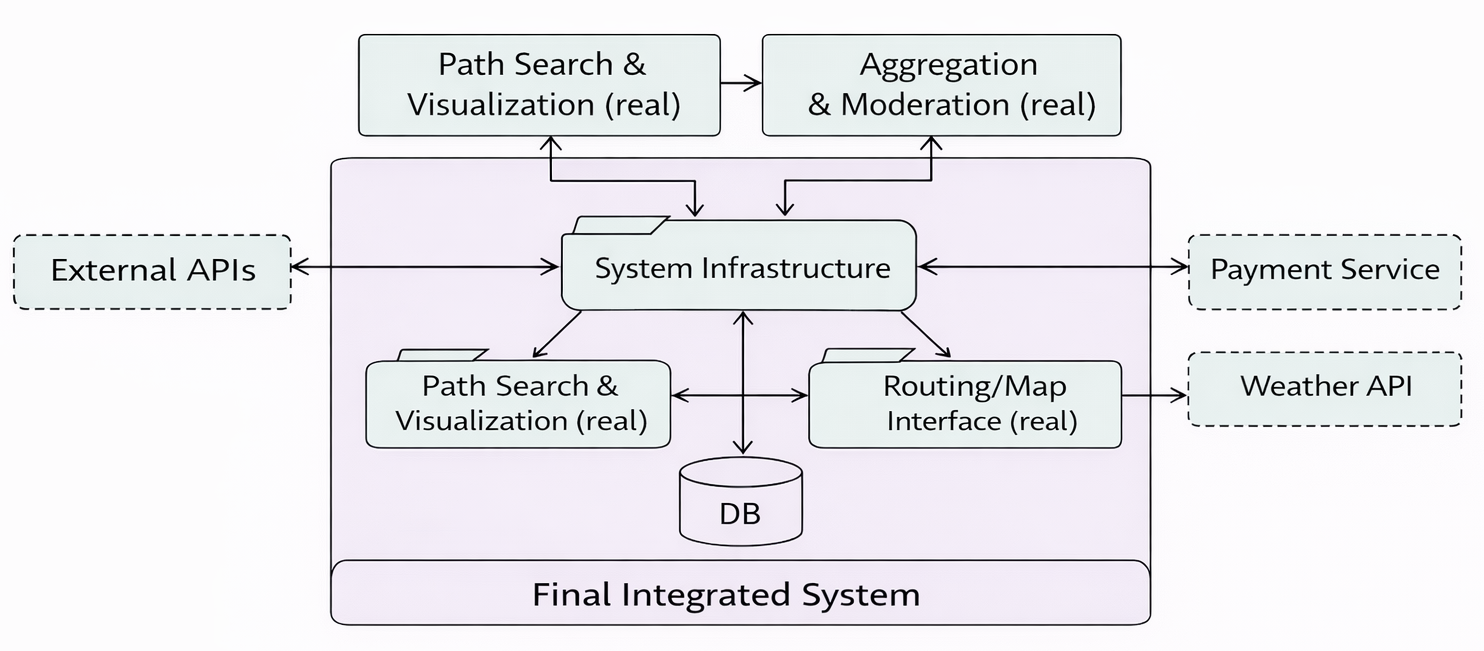
\includegraphics[width=0.95\textwidth]{Figures/final_system}
    \caption{Final system configuration after full integration.}
    \label{fig:final_integration}
\end{figure}

%---------------------------------------------------------

\subsection{Testing Summary}

Testing will be conducted in various levels. Individual modules will be validated by component testing in isolation. Integration testing will validate interactions among subsystems using incremental and thread-based strategies. System tests will verify the behavior of the fully integrated system. This structured testing plan would enhance software quality and minimize integration risks.